\chapter{\IfLanguageName{dutch}{Stand van zaken}{State of the art}}%
\label{ch:stand-van-zaken}

% Tip: Begin elk hoofdstuk met een paragraaf inleiding die beschrijft hoe
% dit hoofdstuk past binnen het geheel van de bachelorproef. Geef in het
% bijzonder aan wat de link is met het vorige en volgende hoofdstuk.

% Pas na deze inleidende paragraaf komt de eerste sectiehoofding.


In dit hoofdstuk wordt de huidige stand van zaken besproken binnen het onderzoeksdomein. Het doel is om een duidelijk beeld te scheppen van de huidige situatie en de bestaande kennis over het onderwerp, en zo een goede basis te vormen voor het verdere verloop van het onderzoek. In dit hoofdstuk wordt er eerst gesproken over het verschil tussen Native, Cross-Platform en Hybrid Development. Het is namelijk noodzakelijk hier een goed beeld van te vormen om de juiste omkadering te geven van beide frameworks. Vervolgens wordt er dieper ingegaan op de Android infrastructuur. Vanwege de verschillen tussen de infrastructuur en werking van React Native en Ionic, is het van belang ook een begrip te hebben van de onderliggende componenten en hun relaties. Daarna zal er een vergelijking gemaakt worden tussen de twee frameworks en zullen er verklaringen of redenen gegeven worden op welke vlakken zij kunnen verschillen en waarom. Tot slot wordt er nog een korte paragraaf gewijd aan de performantie van mobiele applicaties omtrent streaming.

\section{Native vs Cross-Platform vs Hybrid}
\label{sec:native-cross-hybrid}

Voordat er dieper ingegaan wordt op React Native en Ionic, is het belangrijk om ze te situeren binnen Mobile Development. Er kunnen drie grote categorieën onderscheiden worden: Native, Cross-Platform en Hybrid \autocite{Bron12}. Native Development is het ``native'' ontwikkelen van een applicatie voor een specifiek platform. Dit wil zeggen dat een applicatie ontwikkeld wordt in de programmeertaal van het platform, zoals Java of Kotlin voor Android-toestellen en Objective-C of Swift voor iOS-toestellen \autocite{Bron1, Bron11}. Met andere woorden maken deze applicaties gebruik van de officiële ontwikkelingsomgevingen en architecturen van het platform in kwestie. Dit brengt een aantal voordelen met zich mee. Door het gebruik van de native-architectuur en native-UI-tools, kan men profiteren van alle functionaliteiten die het platform aanbiedt. Dat zorgt dan weer voor een optimale performantie en bijgevolg een betere gebruikservaring. Bovendien vereisen ook bepaalde applicaties een native ontwikkeling. Denk hierbij aan programma's die veel resources nodig hebben zoals games \autocite{Bron12}. De keuze voor een native-aanpak brengt echter toch wat nadelen met zich mee. Mobiele applicaties worden echter vaak ontwikkeld met meerdere platformen tegelijk in gedachten, waardoor dezelfde app als het ware dubbel moet worden geprogrammeerd, met als gevolg hogere kosten en development tijdsduur \autocite{Bron12}. Bovendien vereist dit extra kennis van de medewerkers en ontwikkelaars omdat er voor elk platform een andere programmeertaal gebruikt wordt. Kleinere organisaties of start-ups hebben vaak niet altijd voldoende middelen om zulke projecten te financieren. Vandaar dat Cross-Platform en Hybrid Development een oplossing kan bieden.

Het grote voordeel aan Cross-Platform development is dat het steunt op het principe: ``write once, run everywhere'' \autocite{Bron12}. Dit wil zeggen dat ontwikkelaars de applicatie slechts één keer moeten implementeren in een programmeertaal naar keuze en vervolgens kunnen uitrollen op één of meerdere platformen tegelijk zonder hierbij platform-specifieke code te moeten schrijven \autocite{Bron12}. In veel gevallen maakt men gebruik van een framework dat gebaseerd is op talen die ondersteund worden op verschillende platformen, zoals bijvoorbeeld JavaScript. Vervolgens maakt het framework gebruik van een cross-compiler die de code vertaalt naar de platformspecifieke code \autocite{Bron1}. De applicatie heeft bijgevolg een soort van ``native'' look-and-feel, onder meer omdat native-componenten van het toestel hergebruikt worden \autocite{Bron2}. Belangrijk hierbij te vermelden is dat het nog altijd geen echte native-applicatie is vanwege de cross-compiler. Deze tussenstap brengt namelijk een zekere overhead met zich mee, wat kan leiden tot mindere performantie in vergelijking met een echt native-programma \autocite{Bron12}. Bovendien is het niet altijd mogelijk om alle platformspecifieke functionaliteiten te gebruiken \autocite{Bron12}. Wat deze beperkingen zijn, hangt natuurlijk af van framework tot framework. Wat wel vaststaat is dat Cross-Platform Development, in tegenstelling tot Native Development, een pak goedkoper is en sneller verloopt juist vanwege het feit dat er slechts één codebase is.

Tot slot is er nog Hybrid Development. Dit type bevindt zich ergens tussen Native en Cross-Platform Development. Uit verschillende bronnen bleek dat de termen Cross-Platform en Hybrid Development vaak door elkaar worden gebruikt, terwijl er toch een aanzienlijk verschil is tussen beiden \autocite{Bron1, Bron11, Bron12}. Hybrid Development maakt gebruik van webtechnologieën zoals HTML, CSS en JavaScript om een applicatie te ontwikkelen. Er is hier dus opnieuw sprake van herbruikbare code en dus het eenmalig implementeren van de applicatie. Het grote verschil met Cross-Platform Development is dat Hybrid Development de code in een webview of browser-engine van het platform plaatst \autocite{Bron11, Bron1}. Bij Android is dit het WebView component, bij iOS wordt het UIWebView component gebruikt \autocite{Bron4}. Vervolgens wordt de applicatie verpakt in een native container waardoor de applicatie een soort van ``native'' applicatie wordt. Toch valt hierbij op te merken dat de applicatie niet Native is, en ook geen gebruik maakt van native-componenten van het toestel zoals bij Cross-Platform Development \autocite{Bron12, Bron6}. Vanwege dit laatste, kampen zij soms met een inconsistente User Interface, wat natuurlijk een impact kan hebben op de gebruikerservaring \autocite{Bron12}.

Het verschil tussen Cross-Platform en Hybrid development vormt een kernaspect binnen dit onderzoek. Ionic wordt namelijk bestempeld als een Hybrid framework, terwijl React Native een Cross-Platform framework is \autocite{Bron4, Bron1}. Beiden zijn echter mogelijkheden om eenmalig een programma te coderen en vervolgens uit te rollen op meerdere platformen. Beiden zijn bovendien ook niet Native, met de bijhorende impact op de performantie. Hoe de infrastructuur van beide frameworks in elkaar zit, zal in een volgend onderdeel besproken worden.


\section{Android infrastructuur}
\label{sec:android-infrastructuur}

Een belangrijk aspect van dit onderzoek is de infrastructuur van Android. Android is een besturingssysteem ontwikkeld door Google en is gebaseerd op de Linux-kernel \autocite{Bron13}. Het besturingssysteem is open-source en wordt voornamelijk gebruikt op smartphones en tablets. In dit onderdeel wordt de Android infrastructuur besproken en worden de verschillende lagen toegelicht. Dit is belangrijk om een goed beeld te vormen van de onderliggende componenten en hun relaties. Dit zal later in het onderzoek helpen om de verschillen tussen React Native en Ionic beter te begrijpen.

De eerste en bovenste laag van het Android OS is de System Apps of systeemapplicaties \autocite{Bron7, Bron13}. Dit zijn de applicaties die standaard geïnstalleerd zijn op elk Android-toestel. Denk hierbij aan de telefoon-applicatie, de berichten-applicatie, de email-applicatie, enzoverder \autocite{Bron7}. Deze standaardapplicaties hebben verder geen speciale betekenis naast het feit dat ze standaard met het besturingssysteem worden geïnstalleerd. De standaardbrowser die met het toestel komt, kan bijvoorbeeld nog altijd vervangen worden door een andere browser.

De tweede laag noemt het Java API Framework \autocite{Bron7}. Dit is het framework dat ontwikkelaars gebruiken om applicaties te ontwikkelen voor Android. Het bevat een verzameling aan API's geschreven in Java die de features voorstellen van het Android OS. Het bevat een ``View System'' die de ontwikkelaar de mogelijkheid biedt om via buttons, grids, textboxes, enzoverder een User Interface te bouwen \autocite{Bron7, Bron13}. Hierbinnen zit ook een WebView component die een belangrijke rol speelt bij Hybrid Development. Content Providers is een ander onderdeel binnenin het Java API Framework. Dit is een soort mechanisme dat het mogelijk maakt om data van andere applicaties te delen \autocite{Bron7}. Een voorbeeld hiervan is de Contact Provider die een gebruiker toelaat om contactinformatie uit de contacten-app te hergebruiken of zelf te delen met de applicatie, of bijvoorbeeld de Calendar Provider om events of afspraken op de agenda-app op te slaan of te delen. Tot slot zijn er ook nog de verschillende Managers binnen het Java API Framework \autocite{Bron7}. Deze staan in voor de verschillende services die het Android OS aanbiedt. Zo is er de Notification Manager die instaat voor de notificaties en de Location Manager die de locatie van de gebruiker kan bepalen, om enkele voorbeelden te geven.

\begin{figure}
  \centering
  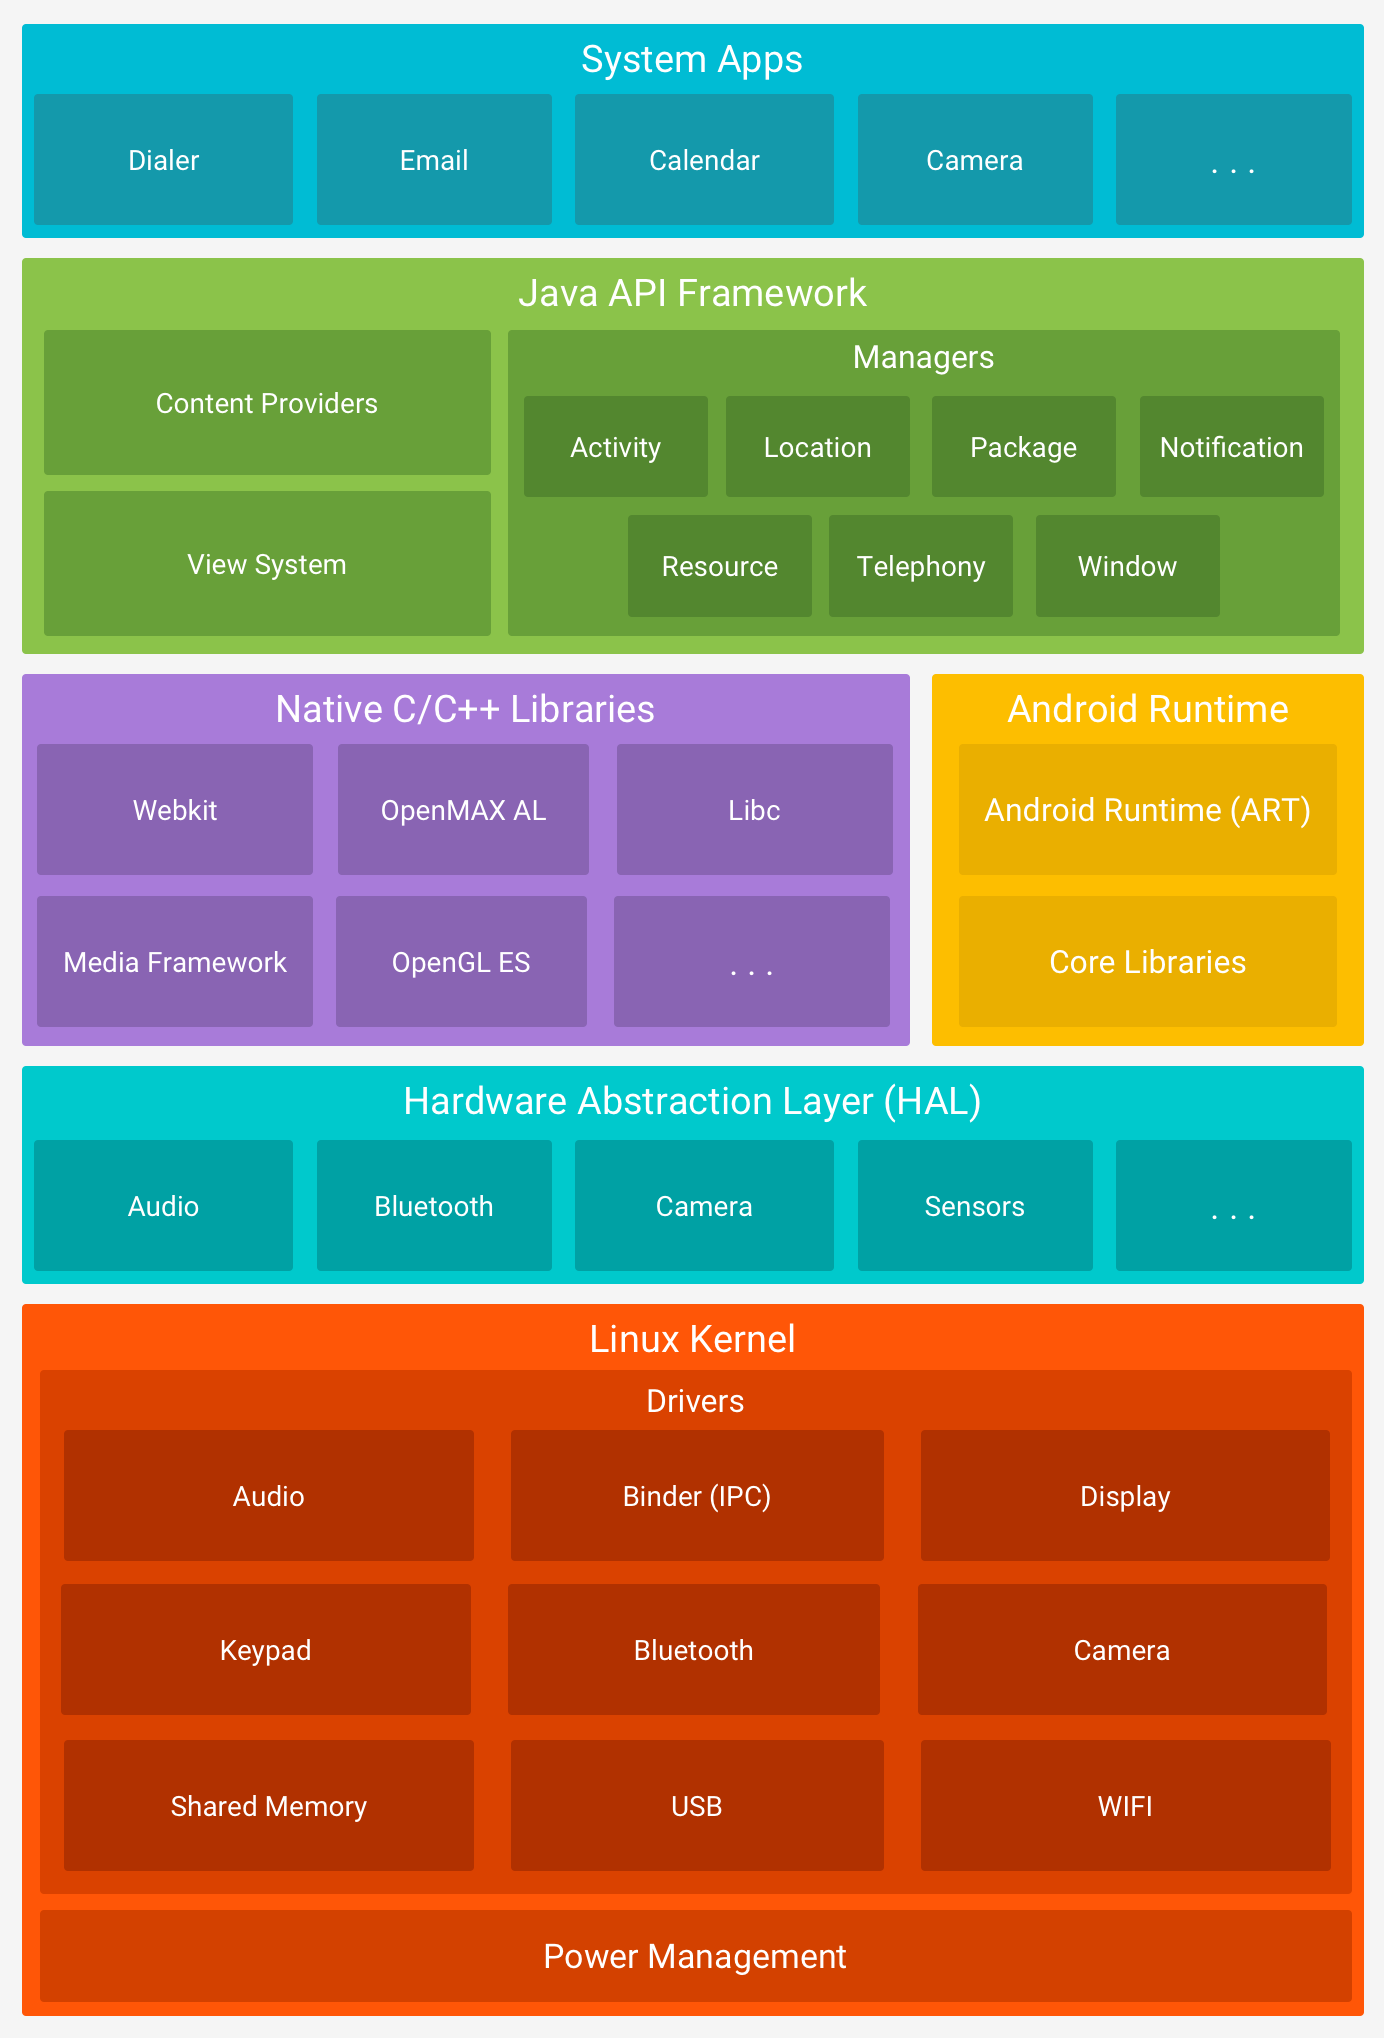
\includegraphics[width=0.9\linewidth]{img/android}
  \caption{Android software stack}
  \label{fig:Android software stack} \autocite{Bron7IMG}
\end{figure}

De volgende laag zijn de Native C/C++ Libraries \autocite{Bron7, Bron13}. Een groot deel van de componenten binnen Android zijn geschreven in C/C++. Android staat toe om de meeste van deze libraries via een Java API te gebruiken. Toch kan het mogelijk zijn dat een ontwikkelaar zijn of haar applicatie in C/C++ wil schrijven. Dankzij deze laag kan er op een native manier in C/C++ geprogrammeerd worden. Om deze laag toch nog wat beter uit te leggen, kan dit geïllustreerd worden aan de hand van een voorbeeld. Stel dat een ontwikkelaar bepaalde 2D of 3D objecten wil gaan renderen in zijn of haar applicatie, bijvoorbeeld bij een video game. De Native C/C++ Libraries bevatten de OpenGL ES library die aan de hand van de C/C++ programmeertaal objecten kan renderen \autocite{Bron7, Bron13}. Toch biedt Android de optie om deze library ook te gebruiken in de bovenstaande Java API Framework laag met behulp van de Java OpenGL API. Zo is het nog steeds mogelijk om via de Java programmeertaal objecten te renderen, maar dan wel met de achterliggende hulp van de OpenGL ES library \autocite{Bron7}. Deze laag kan eigenlijk gebruikt worden om op een meer native manier te programmeren, maar is niet noodzakelijk voor de ontwikkeling van een Android-applicatie. Het kan echter wel meer flexibiliteit bieden.

Vervolgens is er de Android Runtime. Dit is de laag waar de applicaties worden uitgevoerd. Hierbij is de belangrijkste component de Android Runtime (ART) \autocite{Bron7}. Elke applicatie die op het Android OS draait, runt in een eigen proces met een eigen instantie van dit ART component. ART maakt gebruik van Dalvik Executable (.dex) bestanden, een bestandsformaat dat specifiek is ontwikkeld voor Android en geoptimaliseerd is voor mobiele programma's \autocite{Bron14}. Hierin schuilt als het ware de kracht om applicaties die veel resources vereisen, te draaien op een toestel met relatief beperkte kracht. Bovendien biedt ART verschillende runtime functionaliteiten aan zoals Ahead-of-time (AOT) compilatie, Just-in-time (JIT) compilatie en garbage collection mogelijkheden \autocite{Bron7, Bron14}. AOT compilatie zorgt ervoor dat de applicatie gecompileerd wordt voordat deze wordt uitgevoerd, wat de performantie ten goede komt. JIT compilatie daarentegen compileert de applicatie tijdens het uitvoeren, wat de opstarttijd van de applicatie ten goede komt. ART is de opvolger van Dalvik, de vorige runtime van Android. Dalvik maakte alleen gebruik van Just-in-time compilatie, wat de algemene performantie van applicaties soms kon vertragen \autocite{Bron13}. ART is compatibel met Android 5.0 (Lollipop) en is sindsdien de standaard runtime van Android \autocite{Bron7, Bron13}.

Nu komen we bij de voorlaatste laag, namelijk de Hardware Abstraction Layer of kortweg HAL \autocite{Bron7}. Deze laag biedt meerdere interfaces aan om te kunnen communiceren met de onderliggende hardwarelaag. Ze voorkomt dat ontwikkelaars rechtstreeks met de hardware moeten communiceren. Zo hebben de camera, de Bluetooth, de audio, enzoverder allemaal een eigen interface \autocite{Bron7}. Wanneer een API framework uit de bovenliggende laag een bepaalde hardwarefunctie wil gebruiken, zal de HAL de desbetreffende library module inladen. Deze module zal dan de juiste hardwarefunctie aanroepen en de resultaten terugsturen naar het API framework \autocite{Bron7}.

Tot slot is er nog de laatste laag: de Linux Kernel \autocite{Bron7, Bron13}. Dit wordt ook wel gezien als de kern van het Android platform. Een belangrijk proces is dat de ART component deze kernel gebruikt om het geheugen en de processen te gaan beheren \autocite{Bron7, Bron13}. Zaken zoals threading en low-level memory management worden hier geregeld. Vanuit deze laag wordt er uiteindelijk gecommuniceerd met de onderliggende hardware van het toestel om de applicatie te draaien \autocite{Bron13}.

\section{React Native}
\label{sec:react-native}

Dit onderzoek focust zich specifiek op React Native en Ionic. React Native is een open-source framework ontwikkeld door Facebook. Het werd gelanceerd in 2015 en was oorspronkelijk bedoeld voor het programmeren van mobiele applicaties voor iOS-toestellen \autocite{Bron2, Bron1}. In september van datzelfde jaar, enkele maanden na de initiële lancering, was het ook mogelijk om via dezelfde codebase de applicatie te releasen op Android \autocite{Bron1}.

React Native maakt gebruik van het React framework, een ander open source framework, dat aan de hand van JavaScript de mogelijkheid biedt om complexe user interfaces te bouwen \autocite{Bron17}. Een applicatie gebouwd in React Native of React maakt gebruik van JSX-componenten, een combinatie tussen XML en JavaScript code, wat extra flexibiliteit biedt om ook variabelen te declareren binnenin dezelfde componenten \autocite{Bron2}. Bij zowel Android als iOS development bestaat de user interface uit ``Views'' \autocite{Bron18}. Deze vormen de bouwstenen van het scherm van de applicatie en kunnen opgebouwd worden uit meerdere sub-componenten. React Native biedt een groot aantal van die standaardcomponenten aan zoals buttons, inputvelden, sliders, enzoverder. Het principe achter React Native is dat je de Views binnenin Android en iOS kunt gebruiken aan de hand van deze React componenten \autocite{Bron18}. Het \verb|<TextInput>| component binnenin React Native bijvoorbeeld, wordt omgezet naar een \verb|<EditText>| -View in Android en een \verb|<UITextField>| -View in iOS.

De React Native applicatie voor de Proof-of-Concept zal gebruikmaken van het nieuwe Fabric-rendering principe. Eerder maakte React Native gebruik van ``The Bridge'', waarbij de JavaScript code binnenin React werd omgezet naar native-componenten \autocite{Bron1}. Dit principe is helemaal vernieuwd met behulp van Fabric. Om de complexiteit zo laag mogelijk te houden, zal dit uitgelegd worden aan de hand van een voorbeeld die ook werd gegeven door \autocite{Bron17}. In onderstaand voorbeeld hebben we een React-component ``Component'' gedefiniëerd. Deze component bevat een \verb|<View>| component met daarin een \verb|<Text>| component. De code ziet er als volgt uit:

\begin{mdframed}[backgroundcolor=bg]
  \begin{minted}[breaklines]{jsx}
  function Component() {
    return (
      <View>
        <Text>Hello, World</Text>
      </View>
    );
  }
  \end{minted}
\end{mdframed}

In React onderscheiden we twee type componenten: React Composite Components en React Host Components \autocite{Bron15}. React Composite Components zijn de componenten die door de ontwikkelaar zelf gedefinieerd worden, zoals \verb|Component| in bovenstaande code \autocite{Bron16}. React Host Components zijn de standaardcomponenten die React Native aanbiedt, zoals de \verb|<View>| en \verb|<Text>| componenten \autocite{Bron16}. Eens de code moet worden gerendered, zal React deze gedefinieerde componenten eerst omzetten in een React Element Tree. Hierbij worden alle React Host Components, maar niet de zelf gedeclareerde React Composite Components, omgezet naar een boomstructuur van React Elementen \autocite{Bron15}. Een React Element is een JavaScript object dat alle informatie bevat over de component en wat er precies op het scherm moet worden weergegeven \autocite{Bron16}. De reden waarom deze omzetting niet gebeurt voor de zelf gedeclareerde componenten, is omdat deze bestaan uit een verzameling van React Host Components die dan wel weer zullen worden omgezet, of uit andere React Composite Components die op hun beurt ook weer bestaan uit React Host Components. De volledige React boomstructuur kan dus worden vereenvoudigd tot een boomstructuur van enkel React Host Components \autocite{Bron15}.

Tegelijkertijd gaat de Fabric renderer een Shadow Tree aanmaken. Voor elk React Element wordt een React Shadow Node aangemaakt en wordt deze in een gelijkaardige boomstructuur gestoken. Het verschil tussen een React Element en een React Shadow Node is dat de React Element in JavaScript is gedefinieerd en de React Shadow Node in C++ \autocite{Bron16}. Zo bestaat er in het bovenstaande voorbeeld een React Element \verb|<View>| en een React Shadow Node \verb|<ViewShadowNode>|. Nadat de Shadow Tree is aangemaakt, wordt er een commit getriggered \autocite{Bron15}.

\begin{figure}
  \centering
  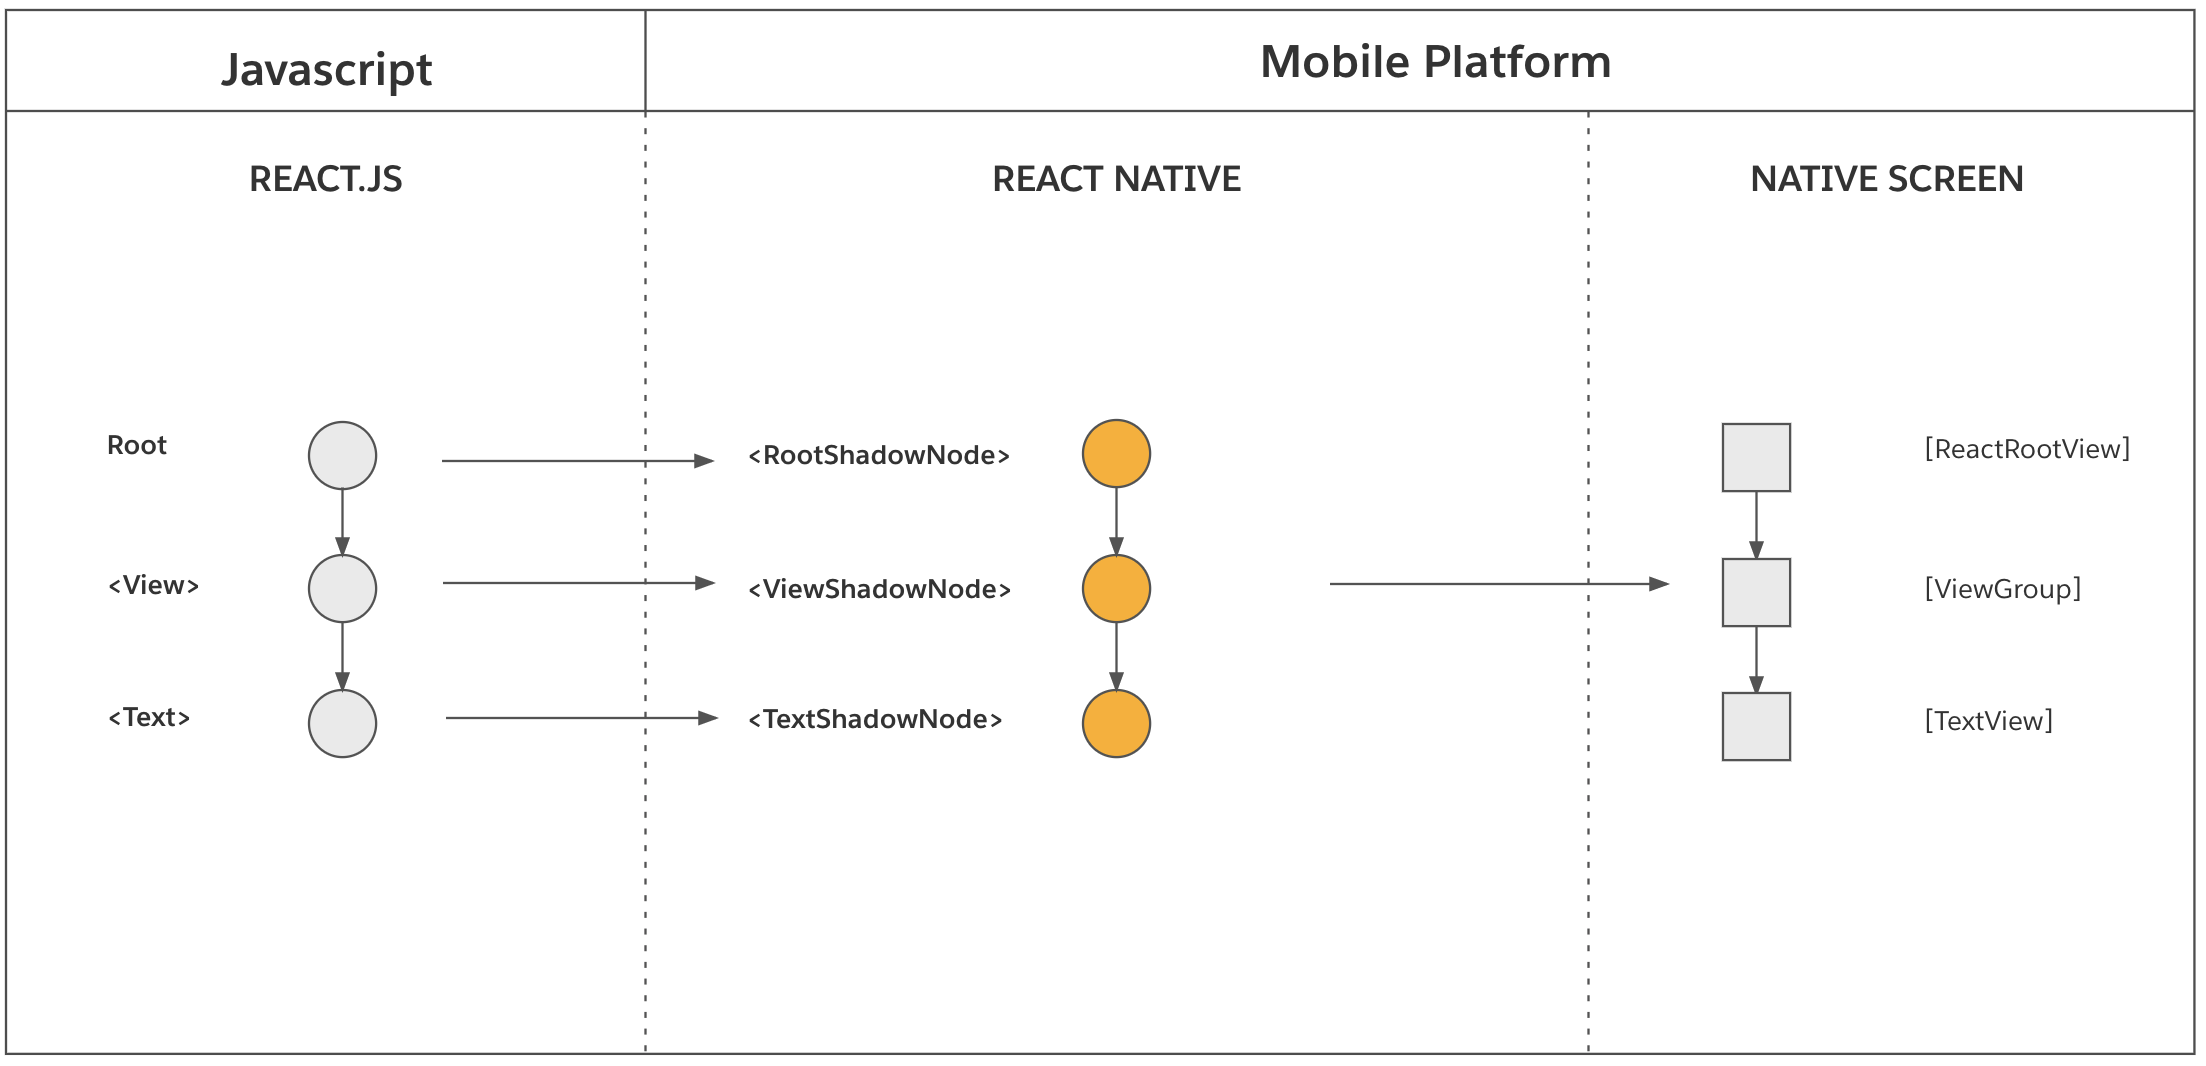
\includegraphics[width=0.9\linewidth]{img/reactNativeRender}
  \caption{Verloop van de React Native rendering}
  \label{fig:Verloop van de React Native rendering} \autocite{Bron15IMG}
\end{figure}

De volgende fase is de Commit fase. Deze bestaat uit twee grote stappen: de Layout Calculation en Tree Promotion \autocite{Bron15}. Bij Layout Calculation wordt alle informatie omtrent de layout, die oorspronkelijk afkomstig is van de React Element Tree, berekend. Zo wordt voor elk component bepaald hoeveel ruimte hij gaat innemen op het scherm \autocite{Bron15}. Bij Tree Promotion wordt de nieuwe Shadow Tree als het ware ``gepromoveerd'' en klaargezet om gemounted te worden \autocite{Bron15}. In eenvoudigere termen betekent dit dat de nieuwe Shadow Tree klaarstaat om op het scherm te worden weergegeven. Zowel de Layout Calculation als de Tree Promotion verlopen asynchroon met elkaar en worden voor het grootste deel in C++ berekend.

De laatste fase, de Mount fase, bestaat uit het renderen van het scherm. Hierbij wordt voor elke React Shadow Node uit de Shadow Tree, samen met de berekende layout informatie, een Host View aangemaakt \autocite{Bron15}. Een Host View is een View die een instantie is van een Android View of een iOS UIView. De React Shadow Nodes worden dus met andere woorden omgezet naar native View-componenten van het desbetreffende platform \autocite{Bron15}. Vandaar de naam ``Native'' in React Native. Deze native View-componenten situeren zich in de Java API Framework laag van de Android OS infrastructuur.

Het is belangrijk hierbij te vermelden dat React Native niet een volledig ``Native'' framework is. Volgens \autocite{Bron3} en \autocite{Bron2} bleek dat er vaak nog wat misconcepties bestaan vanwege deze benaming en wordt het dus vaak foutief bestempeld. Het is en blijft een Cross-Platform framework. Het maakt inderdaad gebruik van native componenten, maar vanwege de cross-compiling tussenstap kan dit niet geplaatst worden onder Native Development.

\section{Ionic}
\label{sec:ionic}

Ionic is net zoals React Native een open source framework. \textcite{Bron8} laat toe om via een webframework naar keuze zoals Angular, React of Vue een applicatie te ontwikkelen die vervolgens kan uitgerold worden op meerdere platformen. Het grote voordeel aan Ionic is dat het gebruik maakt van webtechnologieën zoals HTML, CSS en JavaScript \autocite{Bron8}. Dit heeft als gevolg dat de codebase in Ionic niet alleen kan dienen voor het ontwikkelen van mobiele applicaties, net zoals React Native, maar dat dezelfde codebase ook kan gebruikt worden voor het ontwikkelen van de website zelf. Een ontwikkelaar kan dus zijn of haar applicatie uitrollen op drie platformen tegelijk. Dit onderzoek zal zich specifiek focussen op Ionic in samenwerking met React. Dit vanwege het feit dat React Native ook steunt op React en dat er op deze manier een zeer nauwkeurig beeld kan gegeven worden tussen beide frameworks. Indien er voor een andere framework gekozen zou zijn, zoals bijvoorbeeld Angular of Vue, zou het mogelijk zijn dat bepaalde performantieverschillen eerder te wijten zijn aan de verschillen tussen Angular en React, dan tussen React Native en Ionic.

``Ionic React'' maakt gebruik van dezelfde type React componenten zoals React Native \autocite{Bron8}. Er wordt dus opnieuw gesteund op JSX-componenten, met bovendien extra flexibiliteit van webtechnologieën zoals HTML en CSS. Veel Ionic mobiele applicaties starten eigenlijk vaak als een webapplicatie die vervolgens wordt omgezet naar een mobiele applicatie \autocite{Bron19}. Vroeger gebeurde deze omzetting via Cordova, maar ondertussen heeft Ionic hun eigen versie ontwikkeld, genaamd Capacitor \autocite{Bron19}.

\begin{figure}
  \centering
  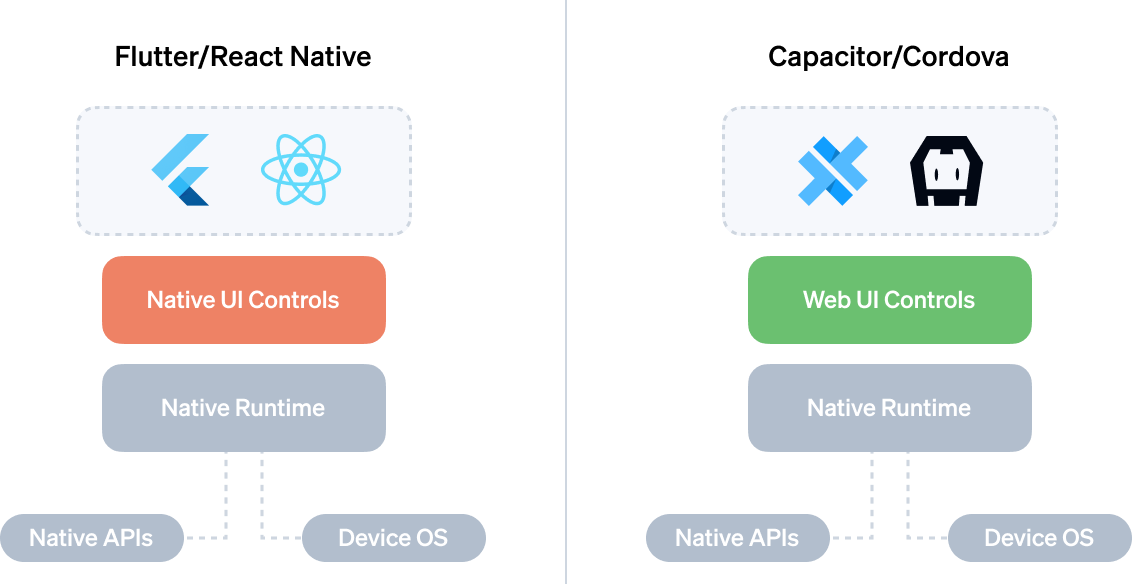
\includegraphics[width=0.9\linewidth]{img/ReactIonic}
  \caption{React Native vs Ionic (Capacitor)}
  \label{fig:React Native vs Ionic (Capacitor)} \autocite{Bron19IMG}
\end{figure}

Via de Capacitor CLI kan de ontwikkelaar met een eenvoudig commando zijn of haar React applicatie laten builden naar een native Android en/of iOS applicatie \autocite{Bron21}. Dit gebeurt door de webapplicatie te bundelen en vervolgens in een native container te plaatsen. Vervolgens wanneer de applicatie wordt geopend, wordt de native webview van het platform aangesproken en de componenten ingeladen \autocite{Bron19}. Het is als het ware een webapplicatie die in een native container draait. In de Android infrastructuur situeert deze container zich, net zoals bij React Native, in de Java API Framework laag. De applicatie kan bovendien nog steeds gebruikmaken van native functionaliteiten zoals de camera, GPS, enzoverder.

Dit laatste aspect maakt Ionic een heel interessant framework voor Hybrid Development en lag ook aan de basis van de keuze om Ionic voor dit onderzoek te gebruiken als Hybrid framework. Zoals eerder aangehaald draaien Hybrid applicaties in een webview of browser-engine van het platform. Om deze reden wordt er soms aangenomen dat deze applicaties niet nuttig zijn omdat typische native functionaliteiten zoals de camera of GPS niet gebruikt kunnen worden. Er wordt vaak gedacht dat deze applicaties slechts enkel en alleen een webapplicatie zijn die in een native container draaien. Ionic biedt echter verschillende plugins aan die het toch mogelijk maken om native API's zoals de GPS en camera aan te spreken. \textcite{Bron22} toont namelijk een lijst van alle beschikbare plugins die Capacitor aanbiedt en steunt daarnaast op een uitgebreide community die zelf plugins ontwikkelen. Dit onderscheidt Ionic van veel andere Hybrid frameworks die enkel webfunctionaliteiten aanbieden en staaft de keuze om Ionic te vergelijken met React Native voor dit onderzoek.

Het verschil tussen React Native en Ionic zit hem voornamelijk in de manier waarop zij de rendering aanpakken. Afbeelding \ref{fig:React Native vs Ionic (Capacitor)} toont een schematische weergave van de verschillen hiervan. React Native gaat de UI-componenten van de applicatie als het ware omzetten naar native View-componenten binnenin de tweede laag van de Android OS infrastructuur: het Java API Framework. Ionic daarentegen maakt gebruik van een WebView-component, een uitbreiding van de native View-component \autocite{Bron23}. De originele webapplicatie wordt samengebundeld en in dit component geplaatst. Beiden situeren zich echter in dezelfde laag van de Android infrastructuur, maar maken elk op een andere manier gebruik van de Android native View-componenten. Het feit dat beide frameworks bovendien ook beschikken over native platformspecifieke functionaliteiten, maakt het interessant om deze twee frameworks met elkaar te vergelijken.


\section{Performantie}
\label{sec:performantie}

Als laatste wordt er nog even kort stilgestaan bij de performantie van video streaming. Video streaming bestaat namelijk uit twee belangrijke processen: encoding en decoding \autocite{Bron25, Bron24}. Bij encoding wordt een videobestand gecomprimeerd en omgezet in een bepaald formaat \autocite{Bron24}. Vanwege de grote bestandsgrootte van mediabestanden, vooral bij video's, vereenvoudigt deze encoding het opslaan en de transmissie ervan. Het is belangrijk hierbij te vermelden dat deze encoding eenmalig gebeurt en dat de video vervolgens in dit formaat wordt opgeslagen. De effectieve grootte van het bestand, samen met de kwaliteit van de video, wordt bepaald door de gebruikte codec \autocite{Bron24}. Enkele voorbeelden van populaire codecs zijn bijvoorbeeld H.264 en HEVC (of H.265) \autocite{Bron25}. Decoding zet vervolgens dit gecomprimeerde bestand weer om in een afspeelbaar formaat op het apparaat tijdens het afspelen van de video \autocite{Bron25, Bron24}. Een belangrijk onderdeel van de decoding is de resolutie van de video. Deze heeft namelijk een grote invloed op de belasting van de CPU en GPU van het toestel \autocite{Bron26}. Als gevolg van een hogere resolutie wordt er meer data ingeladen die vervolgens moet worden verwerkt door de hardware decoder, met de nodige impact op de hardware zelf \autocite{Bron26}. Logischerwijs kan er besloten worden dat indien er een hogere bitsnelheid van de video is, of met andere woorden dat er meer data is, dit een grotere impact zal hebben op de performantie. Deze hogere bitsnelheid kan afhankelijk zijn van de gekozen codec van de video, het aantal beeldjes per seconde, de resolutie van de video en nog andere factoren \autocite{Bron25}. Hoe hier precies mee wordt omgegaan in de Proof-of-Concept, zal in het volgende hoofdstuk besproken worden.




%(nog te schrijven)
%Hierin zal er onder meer gesproken worden over de performantie van mobiele applicaties omtrent streaming en hoe dit een impact kan hebben op de keuze van het framework. De belangrijkste performance-indicatoren zullen hierbij besproken worden.

%Dit hoofdstuk bevat je literatuurstudie. De inhoud gaat verder op de inleiding, maar zal het onderwerp van de bachelorproef *diepgaand* uitspitten. De bedoeling is dat de lezer na lezing van dit hoofdstuk helemaal op de hoogte is van de huidige stand van zaken (state-of-the-art) in het onderzoeksdomein. Iemand die niet vertrouwd is met het onderwerp, weet nu voldoende om de rest van het verhaal te kunnen volgen, zonder dat die er nog andere informatie moet over opzoeken \autocite{Pollefliet2011}.

%Je verwijst bij elke bewering die je doet, vakterm die je introduceert, enz.\ naar je bronnen. In \LaTeX{} kan dat met het commando \texttt{$\backslash${textcite\{\}}} of \texttt{$\backslash${autocite\{\}}}. Als argument van het commando geef je de ``sleutel'' van een ``record'' in een bibliografische databank in het Bib\LaTeX{}-formaat (een tekstbestand). Als je expliciet naar de auteur verwijst in de zin (narratieve referentie), gebruik je \texttt{$\backslash${}textcite\{\}}. Soms is de auteursnaam niet expliciet een onderdeel van de zin, dan gebruik je \texttt{$\backslash${}autocite\{\}} (referentie tussen haakjes). Dit gebruik je bv.~bij een citaat, of om in het bijschrift van een overgenomen afbeelding, broncode, tabel, enz. te verwijzen naar de bron. In de volgende paragraaf een voorbeeld van elk.

%\textcite{Knuth1998} schreef een van de standaardwerken over sorteer- en zoekalgoritmen. Experten zijn het erover eens dat cloud computing een interessante opportuniteit vormen, zowel voor gebruikers als voor dienstverleners op vlak van informatietechnologie~\autocite{Creeger2009}.

%Let er ook op: het \texttt{cite}-commando voor de punt, dus binnen de zin. Je verwijst meteen naar een bron in de eerste zin die erop gebaseerd is, dus niet pas op het einde van een paragraaf.

